\documentclass[aspectratio=169]{beamer}
%
% Choose how your presentation looks.
%
% For more themes, color themes and font themes, see:
% http://deic.uab.es/~iblanes/beamer_gallery/index_by_theme.html
%
\mode<presentation>
{
  \usetheme{default}      % or try Darmstadt, Madrid, Warsaw, ...
  \usecolortheme{default} % or try albatross, beaver, crane, ...
  \usefonttheme{default}  % or try serif, structurebold, ...
  \setbeamertemplate{navigation symbols}{}
  \setbeamertemplate{caption}[numbered]
} 

% Set background to black and text to white
\setbeamercolor{background canvas}{bg=black}
\setbeamercolor{normal text}{fg=white}
\setbeamercolor{frametitle}{fg=white}
\setbeamercolor{title}{fg=white}

% You can continue to set other colors as needed:
\setbeamercolor{item}{fg=magenta} % Color of bullets
\setbeamercolor{subitem}{fg=yellow}
\setbeamercolor{subsubitem}{fg=cyan}
% ...
\setbeamertemplate{frametitle}[default][center]

\usepackage[english]{babel}
\usepackage[utf8]{inputenc}
\usepackage[T1]{fontenc}
\usepackage{graphicx}

% Set larger font for frame title
\setbeamerfont{frametitle}{size=\huge}

\usepackage{emoji}

\begin{document}

\begin{frame}{Syllabus day topics}
\begin{columns}[T]
    \begin{column}[T]{0.5\textwidth}
        \begin{enumerate}
            \item what is a GPU kernel?
            \item why Triton over CUDA?
            \item prerequisites
            \item why use this guide over others?
            \item things to keep in mind during these lectures
            \end{enumerate}
    \end{column}
    \begin{column}{0.5\textwidth}
        
\includegraphics[height=0.8\textheight]{pics/triton-logo.png}
    \end{column}
\end{columns}
\end{frame}

\begin{frame}{what is a GPU kernel?}
\textbf{GPU:} the types of computer processors that we use to make AI, videogames, scientific computing, etc. go BRRRRRR \\
\textbf{GPU kernel:} the function that defines exactly how to do a desired mathematical calculation using an awareness of how GPUs are structured in order to best take advantage of that structure to facilitate going BRRRRRR
\begin{center}
    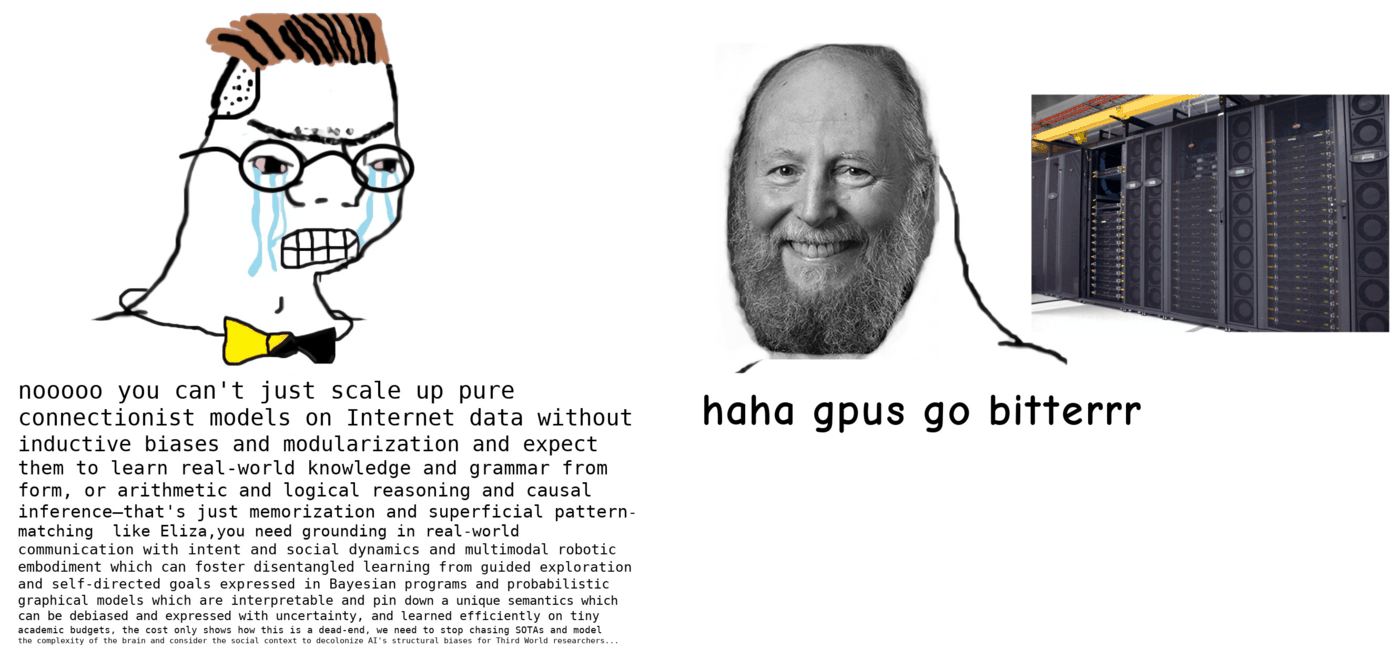
\includegraphics[width=0.7\textwidth]{pics/gpus_go_brrr-2460456025.png}    
\end{center}
\end{frame}

\begin{frame}{why Triton over CUDA?}
\begin{columns}[T]
    \begin{column}[T]{0.4\textwidth}
        
\includegraphics[height=0.2\textheight]{pics/triton-logo.png}
        \begin{itemize}
            \item less popular
            \item open-source
            \item both Nvidia \& AMD
            \item Python
            \item 90\% as fast
            \item linux only
            \item less to learn
            \end{itemize}
    \end{column}
    \begin{column}[T]{0.4\textwidth}
        
\includegraphics[height=0.2\textheight]{pics/nv256n5b1-nvidia-logo-nvidia-logo-free-icon-of-vector-logo-1502684034.jpeg}
        \begin{itemize}
            \item more popular
            \item closed-source
            \item Nvidia GPUs only
            \item C
            \item gold standard for speed
            \item linux or windows
            \item more to learn
            \end{itemize}
    \end{column}
\end{columns}
\end{frame}

\begin{frame}{prerequisites}
required
\begin{itemize}
    \item Python
    \item basic computer hardware concepts (memory, processor, bits vs bytes, floating point operations)
    \item linear algebra
    \item calculus 
    \item common deep learning operations (matmul, softmax, attention, etc.)
    \item PyTorch
\end{itemize}
preferred
\begin{itemize}
    \item some basic but not-universal-among-python-programmer concepts \textit{such as}
    \begin{itemize}
        \item big O notation
        \item compile-time vs run-time
    \end{itemize}
    \item data-structures \& algorithms (leetcode)
\end{itemize}
\end{frame}

\begin{frame}{why use this guide over others?}
guides I used were (links in repo readme)
\begin{itemize}
    \item official triton documentation
    \item Umar Jamil's flash-attention tutorial
    \item GPU Mode's lecture series #14
\end{itemize}
they all some number of the following issues
\begin{itemize}
    \item bugs (kernels straight up didn't pass tests)
    \item slower than PyTorch
    \item assumed you already know CUDA
    \item little to no attempt to explain what was happening
    \item unnecessarily confusing/overcomplicated
    \item primarily one format (text XOR video)
\end{itemize}
\end{frame}

\begin{frame}{things to keep in mind}
\vspace{-1.0in}
\begin{itemize}
    \item i'm not an expert (but I can beat PyTorch)
    \item corrections and elaborations will go in the pinned comment on each video
    \item if you cannot build something you do not understand it! watching/reading is not good enough. you need to go build something sufficiently complex in order to claim comprehension
\end{itemize}
\end{frame}

\end{document}
